\chapter{Modelling heat capacity} \label{chp:models}
    
    To correctly predict the temperature increase of the gas that should be expected when laser energy is input, the heat capacity of argon and hydrogen was modelled. Argon is the current gas used in experiments, while hydrogen is projected to be used for its increased $I_\mathrm{sp}$.

    \section{Equilibrium calculations} \label{sec:equilibrium calcs}
        
        The following seventh order polynomials and their coefficients, from \textcite{mcbrideNASAGlennCoefficients2002}, were implemented in Python. Species of interest were \ce{H}, \ce{H2}, \ce{H+}, \ce{Ar}, \ce{Ar+}, and electrons \ce{e-}. The heat capacity at constant pressure, as well as the temperature dependent part of enthalpy and entropy of each species are given by $C_p^0$, $H^0$ and $S^0$, respectively.

        \begin{equation}
            C_p^0 (T)/R = a_1 T^{-2} + a_2 T^{-1} + a_3 + a_4   T + a_5 T^2 + a_6 T^3 + a_7 T^4
        \end{equation} 
        
        \begin{equation}
            H^0 (T)/RT = -a_1 T^{-2} + a_2 \ln(T)/T + a_3 + a_4 T / 2 + a_5 {T^2}/3 + a_6 {T^3}/4 + a_7 {T^4}/5 + b_1/T
        \end{equation}
        
        \begin{equation}
            S^0(T)/R = -a_1 T^{-2}/2 - a_2 T^{-1} + a_3\ln(T) + a_4   T + a_5 {T^2}/2 + a_6 T^3/3 + a_7 T^4/4 + b_2
        \end{equation}

        Indeed, plasma temperatures of about \qty{15000}{K} enable us to treat it as singly ionized. [Add graph]

        Next, the functions for entropy and Gibbs free energy, both per \unit{kmol}, were implemented. These values depend on temperature and pressure. 
        
        \begin{equation}
            \bar s_i (T, p_i) = \bar s_i^0 (T) - \bar R \ln \frac{y_i p}{p_{ref}}
        \end{equation}

        \begin{equation}
            \bar g = \bar h - T \bar s
        \end{equation}

        Considering the mole fractions of the different species, different expressions for the two gasses are found:

        For Argon,
        \begin{equation}
            potato 1
        \end{equation}

        For Hydrogen,
        \begin{equation}
            potato 2
        \end{equation}


        Plotting the Gibbs energy of the hydrogen mixture as a function of x, for different pressures:

        \begin{figure}[!ht]
            \centering
            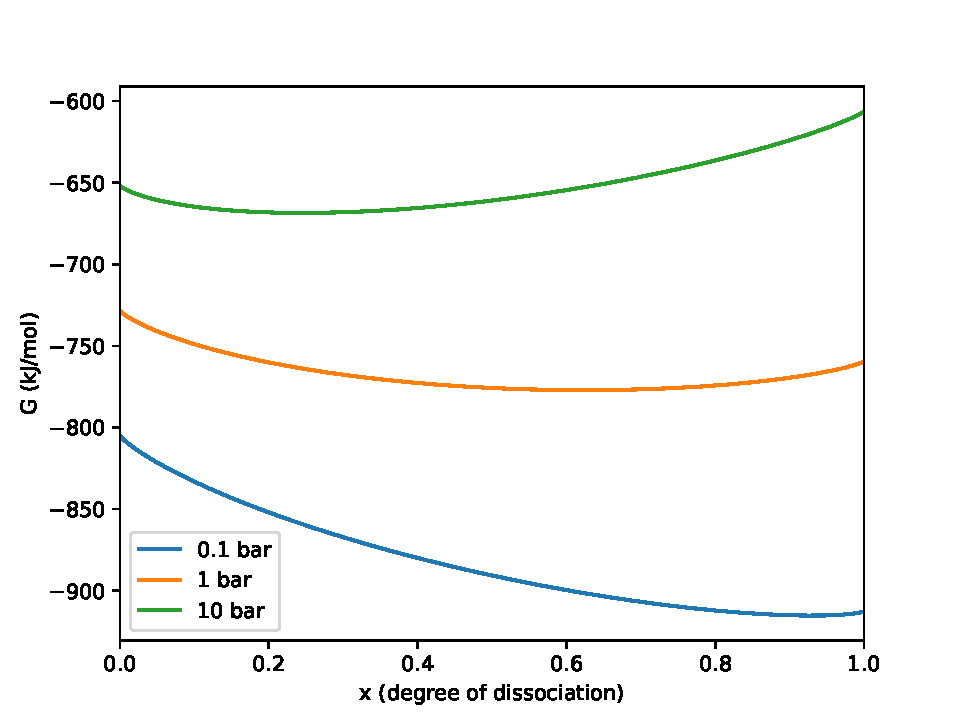
\includegraphics[width=0.7\textwidth]{assets/2 models/Gibbs.pdf}
            \caption{Gibbs free energy (G) plotted against the degree of dissociation (x) of hydrogen under three different pressures}
            \label{fig:Gibbs}
        \end{figure}

        A mixture will reach equilibrium at the minimum of the Gibbs energy.

        Finally, the calculated $C_p$ values were then validated against values from CEA \cite{CEARUNRev4}. 
        
        \begin{figure}[!ht]
            \centering
            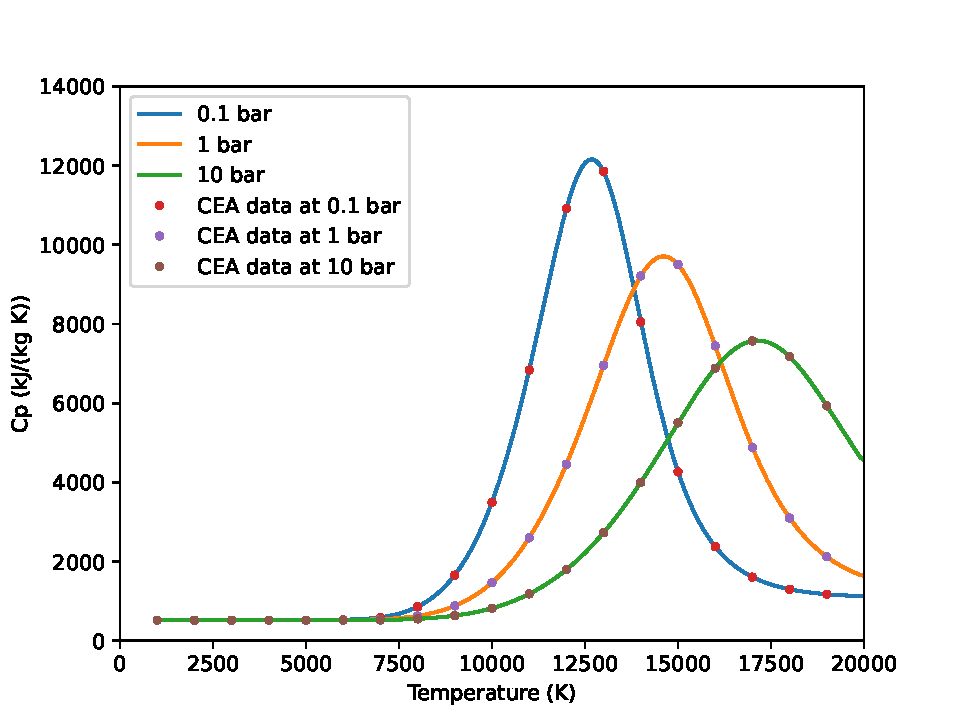
\includegraphics[width=0.7\textwidth]{assets/2 models/Cp_compare.pdf}
            \caption{Comparing calculated $C_p$ values of hydrogen to those from CEA}
            \label{fig:Cp_compare}
        \end{figure}

        The discrepancy can be explained by our initial assumption that at these temperatures, hydrogen dissociates but does not ionize, while argon singly ionizes.

    \section{Test problem for heat addition}

        With these variable heat capacities, a test problem can be solved, giving a preliminary 0D model of an LTP engine.

        Bla bli